\documentclass[12pt]{article}
 
\usepackage[landscape,margin=0.5in,top=0.5in,bottom=0.5in,a4paper]{geometry}
\usepackage{amsmath,multicol,titlesec,graphicx,listings}

\usepackage[utf8]{inputenc}
\titlespacing{\section}{0pt}{5pt}{0pt}
\titlespacing{\subsection}{0pt}{5pt}{0pt}
\titlespacing{\subsubsection}{0pt}{5pt}{0pt}
\setlength{\parindent}{0pt}
\pagenumbering{gobble}
\titleformat*{\section}{\large\bfseries}
\titleformat*{\subsection}{\bfseries}
\setlength{\columnseprule}{1pt}
 
\begin{document}
\raggedright
\begin{multicols}{4}

\subsection{Condensadors}

\underline{Capacitat} $\varepsilon \varepsilon_0 A / d$ \\
\underline{Càrrega} $q = CV$ \\
\underline{Energia electroestàtica}: $W = E = \frac{1}{2}CV_C^2 = \frac{1}{2}\frac{Q^2}{C}$

\section{Diodes}

\underline{Eq. de Shockley}: $I = I_0 \left( e^{\frac{V}{\eta V_\tau}} -1 \right)$ \\
$V_\tau = \frac{k_BT}{e}, \eta \approx 1, I_0 = \text{corrent saturació inversa}$ \\
\underline{Eq. de Planck}: $E = h \nu$ \\
$h = 6,62 \times 10^{-34}$ [Js]

\section{Transistors}

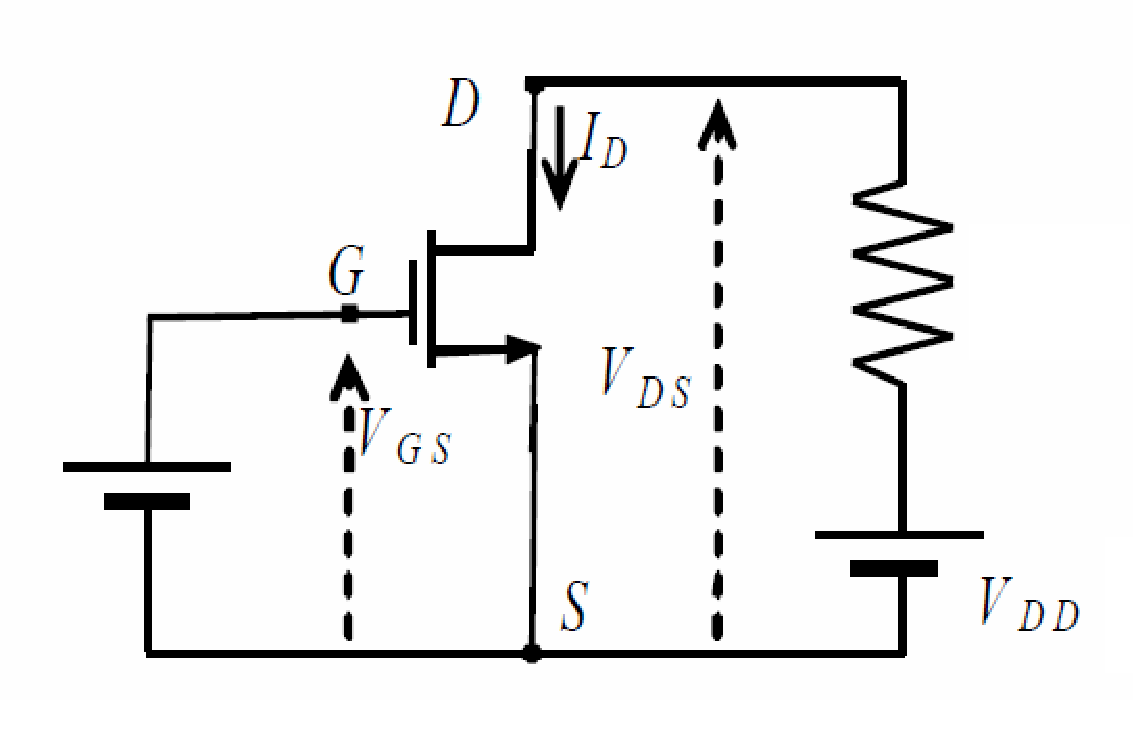
\includegraphics[width=\linewidth]{Auxiliar/Figura1.pdf}

\subsection{Transistors NMOS}

\texttt{if ($V_{GS} > V_T$) }\\
\texttt{ if ($V_{DS} > V_{GS} - V_T$) (1)} \\
\texttt{ else (2)} \\
\texttt{else (3)} \\
\texttt{ } \\
(1) \underline{zona de saturació}: $I_D = \frac{\beta}{2} (V_{GS}-V_T)^2$ \\
(2) \underline{zona lineal (óhmica)}: $I_D = \beta \left[ \left( V_{GS} - V_T \right) V_{DS} - \frac{V_{DS}^2}{2} \right]$ \\
(3) \underline{zona de tall}: $I_D = 0$

\subsection{Transistors PMOS}

\texttt{if ($V_{GS} < V_T$) }\\
\texttt{ if ($V_{DS} < V_{GS} - V_T$) (1)} \\
\texttt{ else (2)} \\
\texttt{else (3)} \\
\texttt{ } \\
(1) \underline{zona de saturació}: $I_D = \frac{\beta}{2} (V_{GS}-V_T)^2$ \\
(2) \underline{zona lineal (óhmica)}: $I_D = \beta \left[ \left( V_{GS} - V_T \right) V_{DS} - \frac{V_{DS}^2}{2} \right]$ \\
(3) \underline{zona de tall}: $I_D = 0$

\section{Retras i potència en circuits digitals}

Interruptor de: \\
\qquad càrrega $C \approx 1 [F]$ \\
\qquad tensió d'alimentació $V_{DD}$ \\
\qquad relació d'activitat $p$ \\
\qquad corrent $I$ \\
\qquad clock $f_C$ \\
\underline{Potència dinàmica de càrrega}: $P_{\text{dinàmica}} = p f_C C V_{DD}^2$ \\
\underline{Potència estàtica}: $P_{\text{estàtica}} = I V_{DD}$ \\
\underline{Potència dissipada}: $P = P_{\text{dinàmica}} + P_{\text{estàtica}}$ \\
\underline{Energia de commutació}: $E = C V_{DD}^2 + \frac{I V_{DD}}{p f_C}$

\section{Varis}

\underline{Nombre d'Avogadro}: $N_A = 6,22 \times 10^{23}$ \\

\end{multicols}
\end{document}
